\chapter{Metodologia}\label{cap:metodologia}

Neste capítulo é descrita a sequência de etapas que serão realizadas neste trabalho para que os objetivos de pesquisa sejam alcançados. 

Iniciaremos com uma revisão bibliográfica para conhecer o estado da arte e depois definir as características que representarão os padrões a serem classificados. Em seguida, faremos um levantamento das classes relevantes para classificação de terrenos neste tipo de imagens aéreas, considerando a relevância destes para a problemática em questão.

Em um momento posterior será feito um levantamento na literatura sobre algoritmos e métodos comumente usados para a segmentação das imagens por tipo de terreno. Por fim, experimentos serão realizados para identificar os métodos (vetor de características e técnicas de aprendizado) com maior taxa de acurácia para o problema específico de segmentação por tipo de terreno em imagens aéreas da região de floresta amazônica.

Essa segmentação tem por objetivo aferir a eficiência de uma detecção de anomalias utilizando aprendizado em multiníveis, ou seja, observar se a pré-classificação dos terrenos e características geográficas encontrados nas imagens podem auxiliar na determinação de técnicas e características específicas de detecção de anomalias próprias de cada tipo de terreno.

A última etapa experimental é testar e comparar algoritmos para detecção de anomalias nas regiões segmentadas das imagens, admitindo a possibilidade de necessitarmos extrair diferentes características em relação à fase de segmentação dos experimentos. O objetivo desta etapa é encontrar as técnicas para detecção de anomalias em imagens aéreas específicas para cada tipo de terreno, completando o processo de busca por anomalias na imagem como um todo. O diagrama apresentado na figura \ref{fig:metDiagrama} explana o arcabouço utilizado no trabalho.

\begin{figure}[h]
    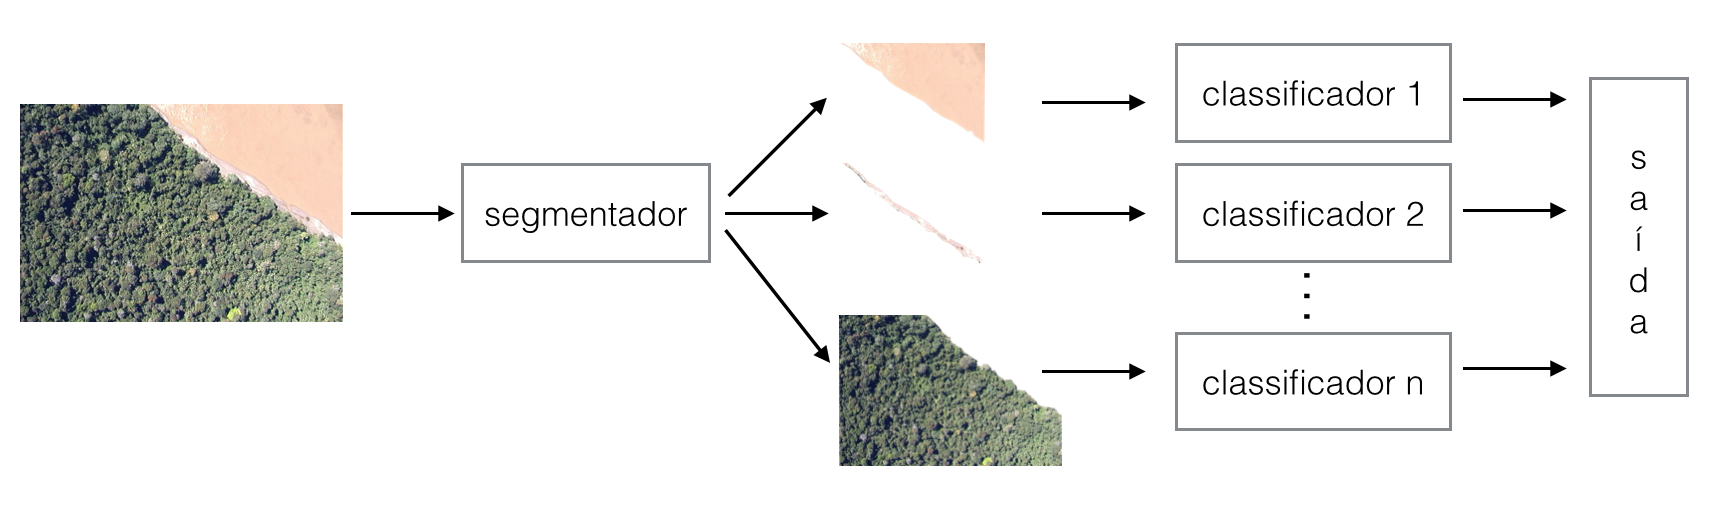
\includegraphics[width=\textwidth]{imgs/diagrama}
    \caption{Método a ser desenvolvido para detecção de anomalias em imagens aéreas da floresta amazônica}
    \label{fig:metDiagrama}
\end{figure}

%A bibliografia utilizada é composta por artigos e livros sobre a detecção de padrões em imagens e de sensoriamento remoto, área das geociências com bastante conhecimento em processamento e classificação de imagens aéreas.

Durante o desenvolvimento do trabalho, artigos serão submetidos com os resultados intermediários, para divulgação e validação junto à comunidade científica. Por fim, a dissertação final do programa de mestrado será redigida, contendo o resultado dos experimentos, seus êxitos e problemas encontrados.